\section{\Large PROBLEM SET 6}

\subsection{Problem 1 - Complete the modeling and verification of perturbation torques as described in the previous pset}

In the previous problem set, the magnetic torque was implemented successfully, but the aerodynamic and solar 

\subsection{Problem 2 - Compute the attitude control error even if a controller is not implemented yet. The attitude control error represents the rotation between the desired and actual attitude. Plot the attitude control error and give its interpretation. Note that this step requires the definition and computation of the desired or nominal or target attitude of the spacecraft. In general, this can be expressed in body or principal axes.}

Recall that the mission for the Aqua satellite requires the instruments on the bottom of the craft to be Earth-pointing. With the selected body axes, this means that the desired attitude expressed as a rotation matrix from the RTN frame to the body frame is described as follows.

\begin{equation*}
    \boldsymbol{\bar{R}}_{RTN \rightarrow x'y'z'} = \begin{bmatrix}
        0 & 1 & 0 \\ 0 & 0 & 1 \\ 1 & 0 & 0
    \end{bmatrix}
\end{equation*}

To get the desired orientation of the principal frame we use the rotation described in Section \ref{sec:principal_inertia_def_and_calc}. Using Equation \ref{eq:desired_principal_RTN}, the desired attitude of the principal frame with respect to the RTN frame can computed, where $\boldsymbol{A}$ is represented by $\boldsymbol{R}_{xyz \rightarrow x'y'z'}$.

\begin{equation} \label{eq:desired_principal_RTN}
    \boldsymbol{\bar{R}}_{RTN \rightarrow xyz} = \boldsymbol{R}_{xyz \rightarrow x'y'z'}^T \boldsymbol{\bar{R}}_{RTN \rightarrow x'y'z'}
\end{equation}

Therefore, at each step in the simulation, the desired attitude with respect to the ECI frame is computed using Equation \ref{eq:desired_principal_ECI}.

\begin{equation} \label{eq:desired_principal_ECI}
    \boldsymbol{\bar{R}}_{ECI \rightarrow xyz} = \boldsymbol{\bar{R}}_{RTN \rightarrow xyz} \boldsymbol{R}_{ECI \rightarrow RTN}
\end{equation}

The error between the current and desired attitude can be represented by a rotation from the current attitude to the desired attitude. This rotation can be computed using Equation \ref{eq:error_rotation}

\begin{equation} \label{eq:error_rotation}
    \boldsymbol{R}_{\text{error}} = \boldsymbol{R}_{xyz \rightarrow \overline{xyz}} = \boldsymbol{\bar{R}}_{ECI \rightarrow xyz} \boldsymbol{R}_{ECI \rightarrow xyz}^T
\end{equation}

Aligning the satellite initially with this initial condition but giving it no initial angular velocity should yield an evolution of the error that mostly resembles a linear increase in the angle $\theta$. This is because this angle represents the error about the desired 2-axis, which in our desired alignment corresponds to the N-axis in the RTN frame. In the absence of disturbances the only apparent rotation should be that of the RTN frame as the satellite moves in its orbit. Figure \ref{fig:attitude_error_no_dist} corroborates this interpretation. An issue occurs with a singularity at $\theta = 90^\circ$, causing the signs of the other two angles to flip. The general behavior, however, remains the same under this consideration.

\begin{figure}[H]
    \centering
    \captionsetup{ justification = centering }
    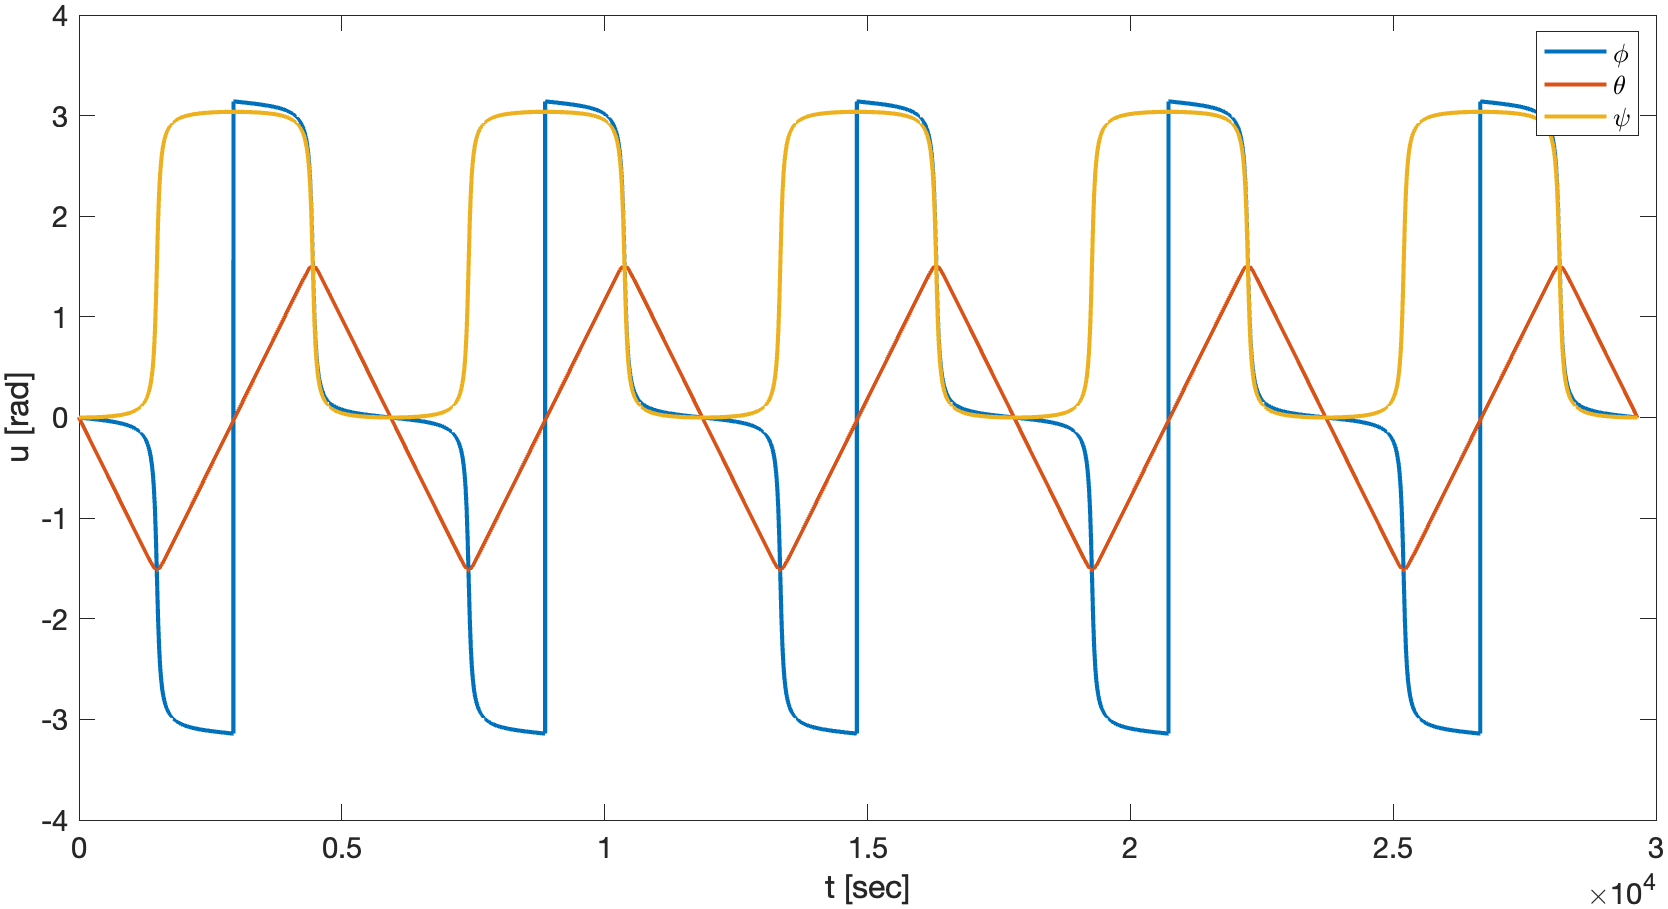
\includegraphics[width = 12cm]{Images/PS6/attitude_error_no_dist.png}
    \caption{312 Euler Angle Parameterization of the Rotation Error in the Absence of Disturbance Torques}
    \label{fig:attitude_error_no_dist}
\end{figure}

\subsection{Problem 3 - Note that the attitude control error represents a rotation matrix (DCM) which quantifies how far the actual attitude is from the true attitude. You can use any parameterization to plot the attitude control errors corresponding to this DCM. Give interpretation of the attitude control errors given the applied disturbances.}

In the presence of disturbances, the motion will be similar during a large portion of the first orbit, but the presence of oscillatory moments throughout each orbit will slowly change the angular velocity vector of the spacecraft, causing the evolution to become less linear and more oscillatory. The period of these oscillations will also grow shorter over time. The simulation results are shown in Figure \ref{fig:attitude_error_dist}.

\begin{figure}[H]
    \centering
    \captionsetup{ justification = centering }
    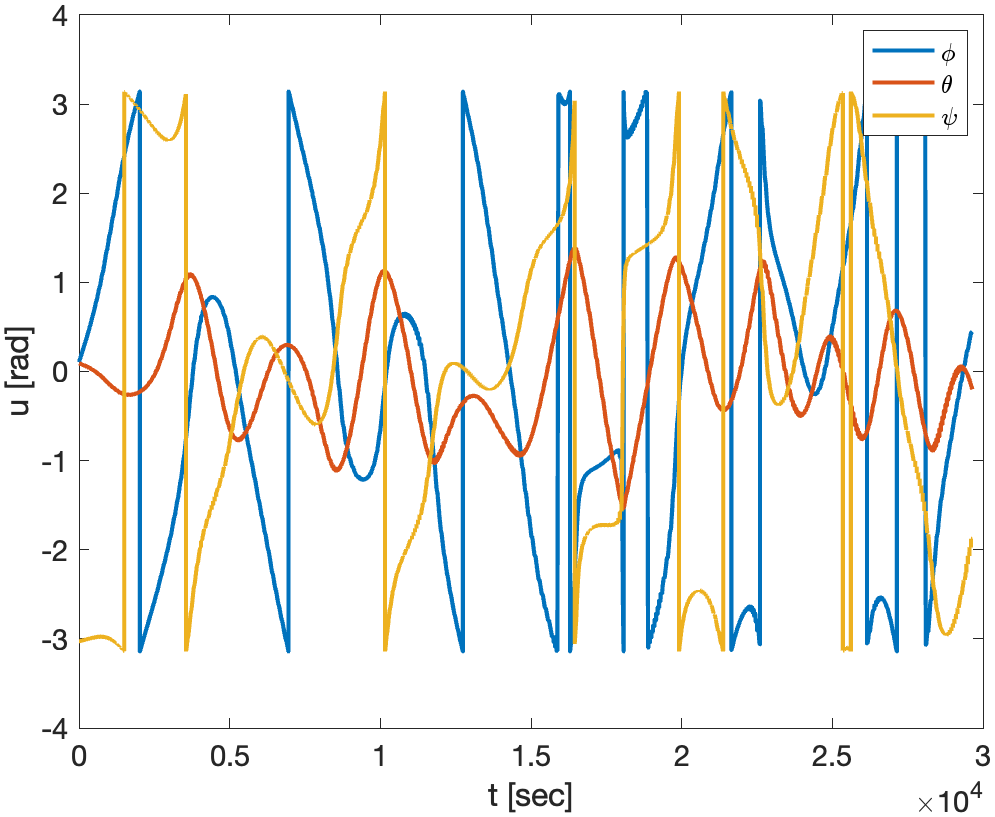
\includegraphics[width = 12cm]{Images/PS6/attitude_error_dist.png}
    \caption{312 Euler Angle Parameterization of the Rotation Error in Presence of Disturbance Torques}
    \label{fig:attitude_error_dist}
\end{figure}

\subsection{Problem 4 - You can now start modeling the Simulink spacecraft subsystem which is what the satellite believes is happening (on-board). Initially, the sensors provide ideal measurements (no bias or noise). Just use an empty box for those. The outputs of the sensors are measurements which are used for attitude determination. These measurements are computed from the reference truth or oracle.}

The sensors onboard the satellite that return reference vectors corresponding the location or direction of physical things in space are star trackers and magnetometers. For the sake of proving the functionality of the deterministic and statistical methods for attitude determination, it was deemed sufficient to only use star tracker measurements. The model shown in Figure \ref{fig:star_tracker_meas} depicts the simulated generation of star tracker measurements from a set of randomly selected ground truth unit vectors. Each component of the measurement vectors are perturbed by a random number ranging from -1 to 1 that is scaled by a so called "noise factor." Here, this factor is chosen to be 0.

\begin{figure}[H]
    \centering
    \captionsetup{ justification = centering }
    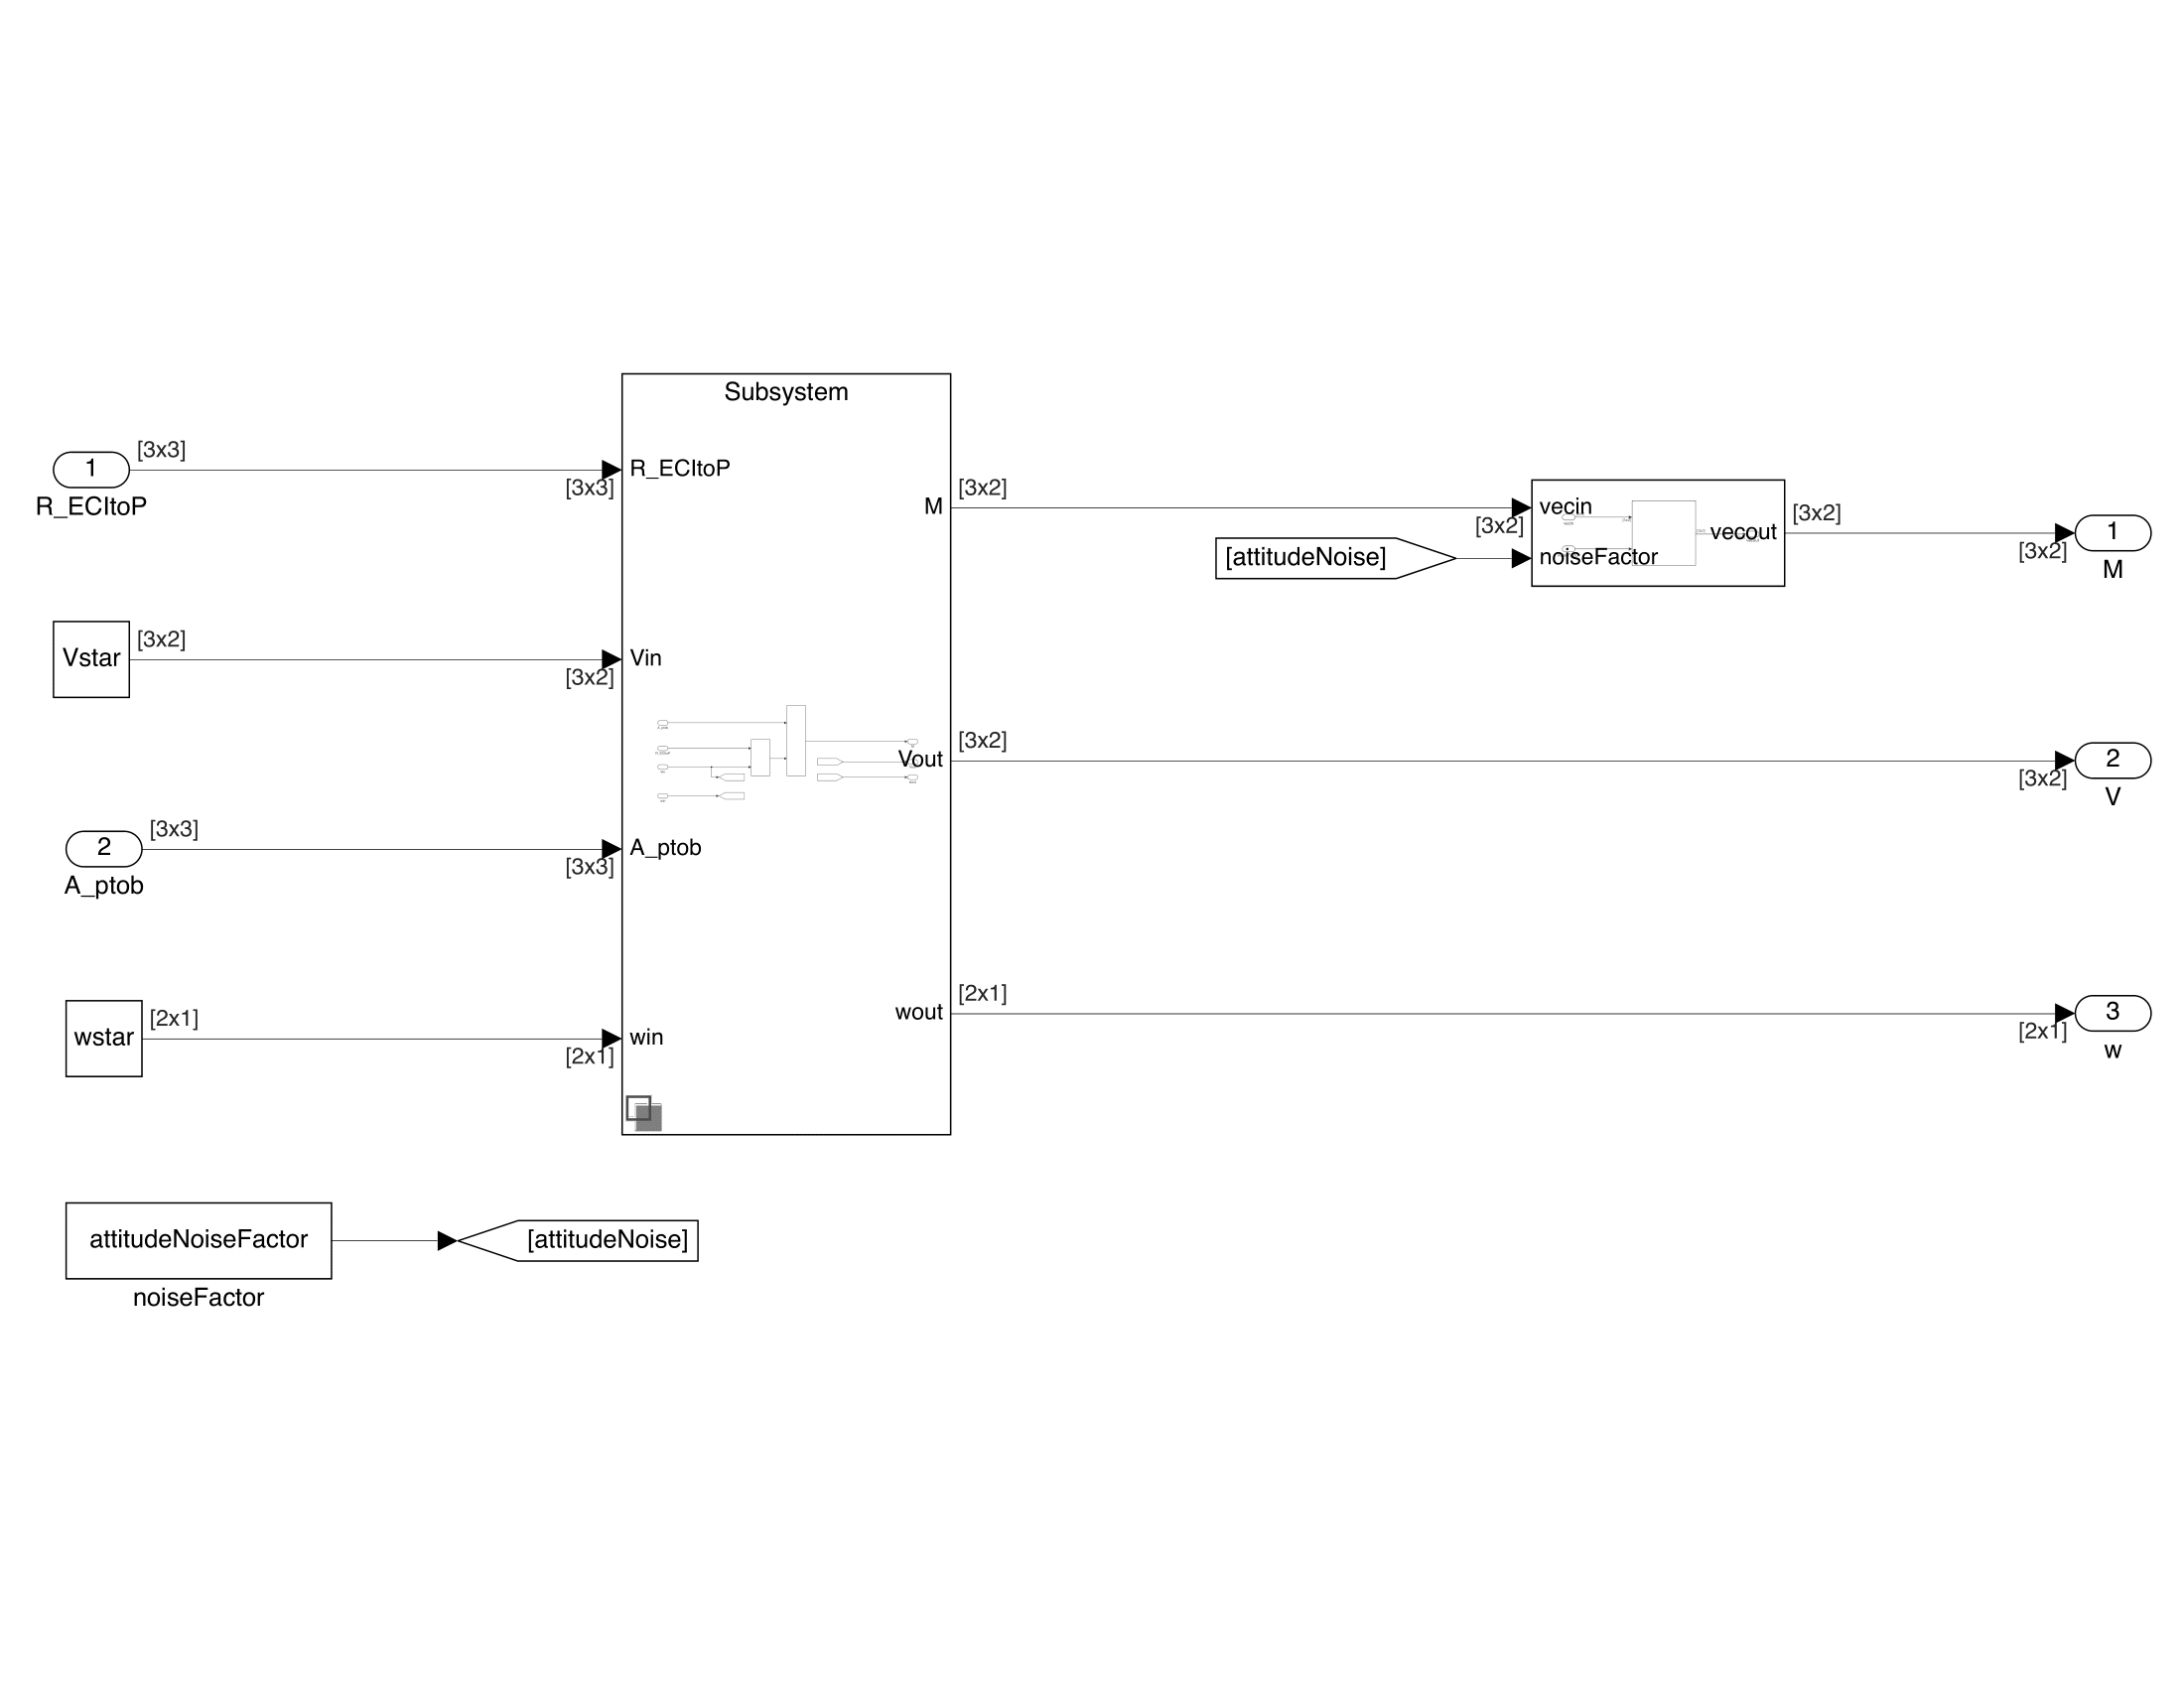
\includegraphics[trim={0.25cm 3cm 0.25cm 3cm},clip,width = 15cm]{Images/PS6/raw_meas_star.png}
    \caption{Model for Star Tracker Measurement Generation}
    \label{fig:star_tracker_meas}
\end{figure}

The model used to rotate the ground truth vectors into the body frame is seen in Figure \ref{fig:ground_truth_to_meas}.

\begin{figure}[H]
    \centering
    \captionsetup{ justification = centering }
    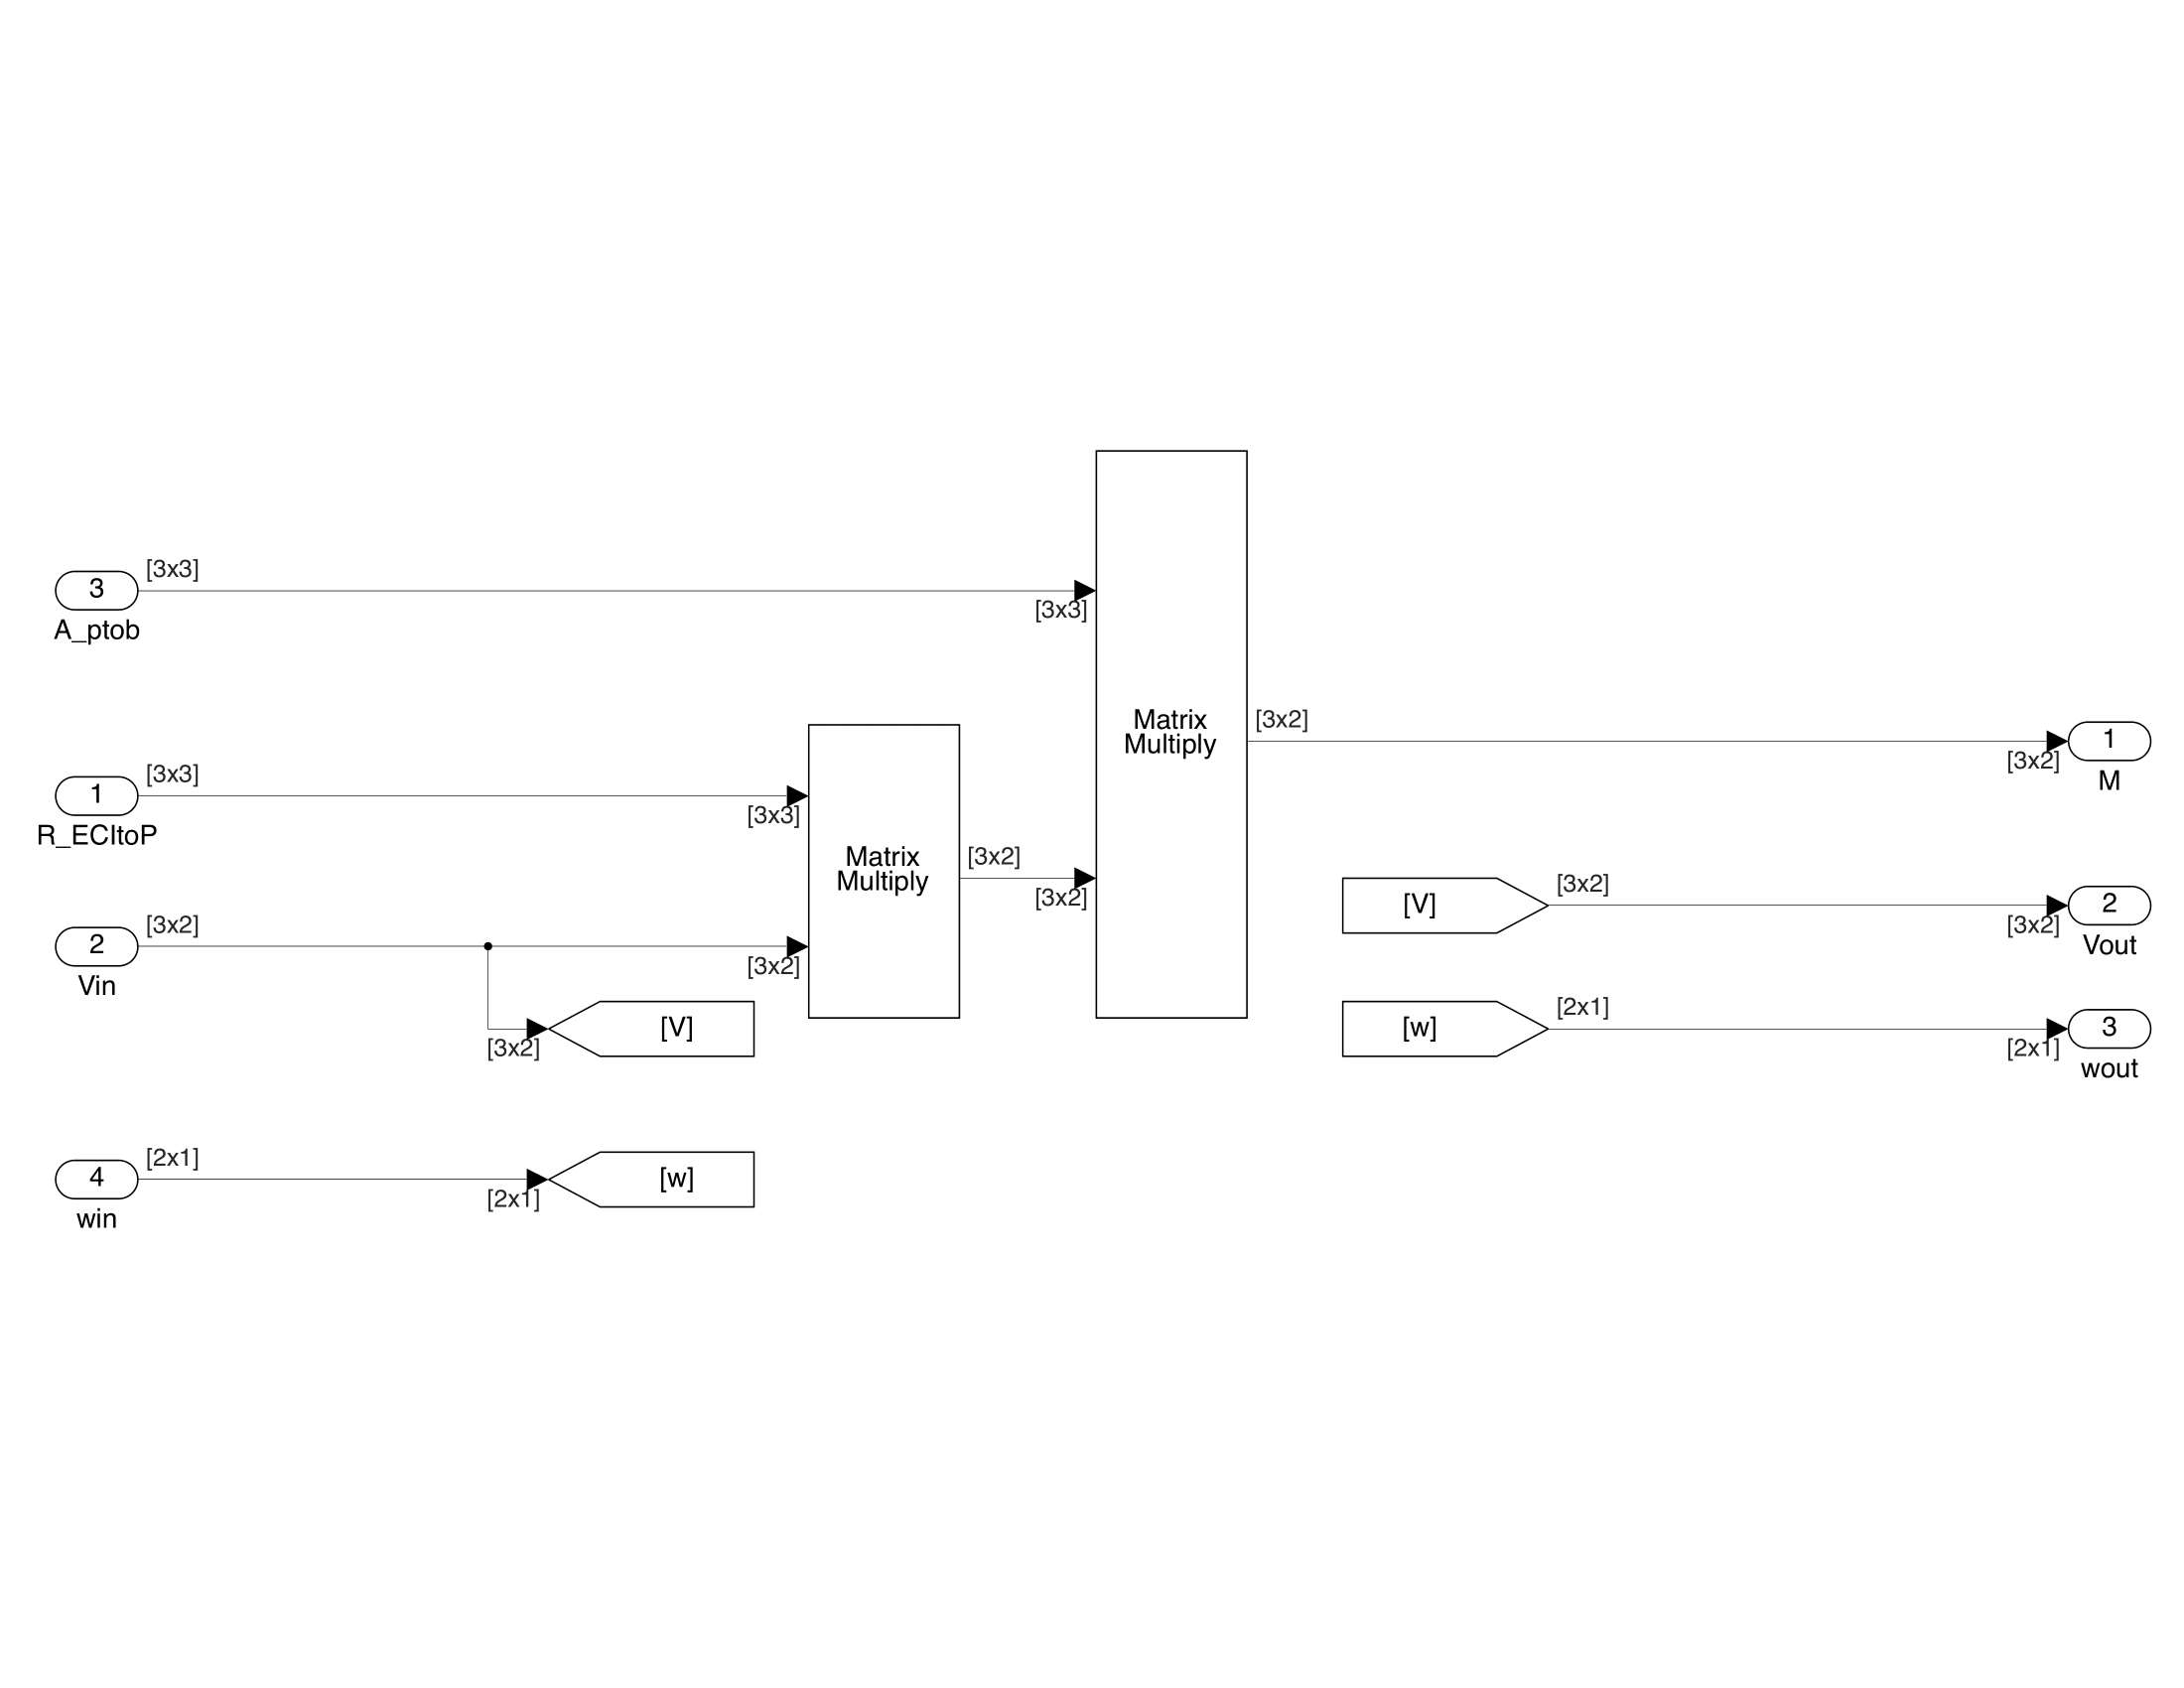
\includegraphics[trim={0.25cm 3cm 0.25cm 3cm},clip,width = 15cm]{Images/PS6/ground_truth_to_meas.png}
    \caption{Ground Truth to Measurement Model}
    \label{fig:ground_truth_to_meas}
\end{figure}

In addition to this, a system was created that would feed through sets of measurements that contain 3 or more vectors, but will create a triad if only two measurements are available. Additionally, for the case where only two measurements are available, the errors can be mitigated by creating two fictitious measurements first before generating the triad that ultimately gets fed into the deterministic determination algorithm. The feed through model can be seen in Figure \ref{fig:feedthrough_meas} whereas the fictitious measurement model can be seen in Figure \ref{fig:fictitious_meas}.

\begin{figure}[H]
    \centering
    \captionsetup{ justification = centering }
    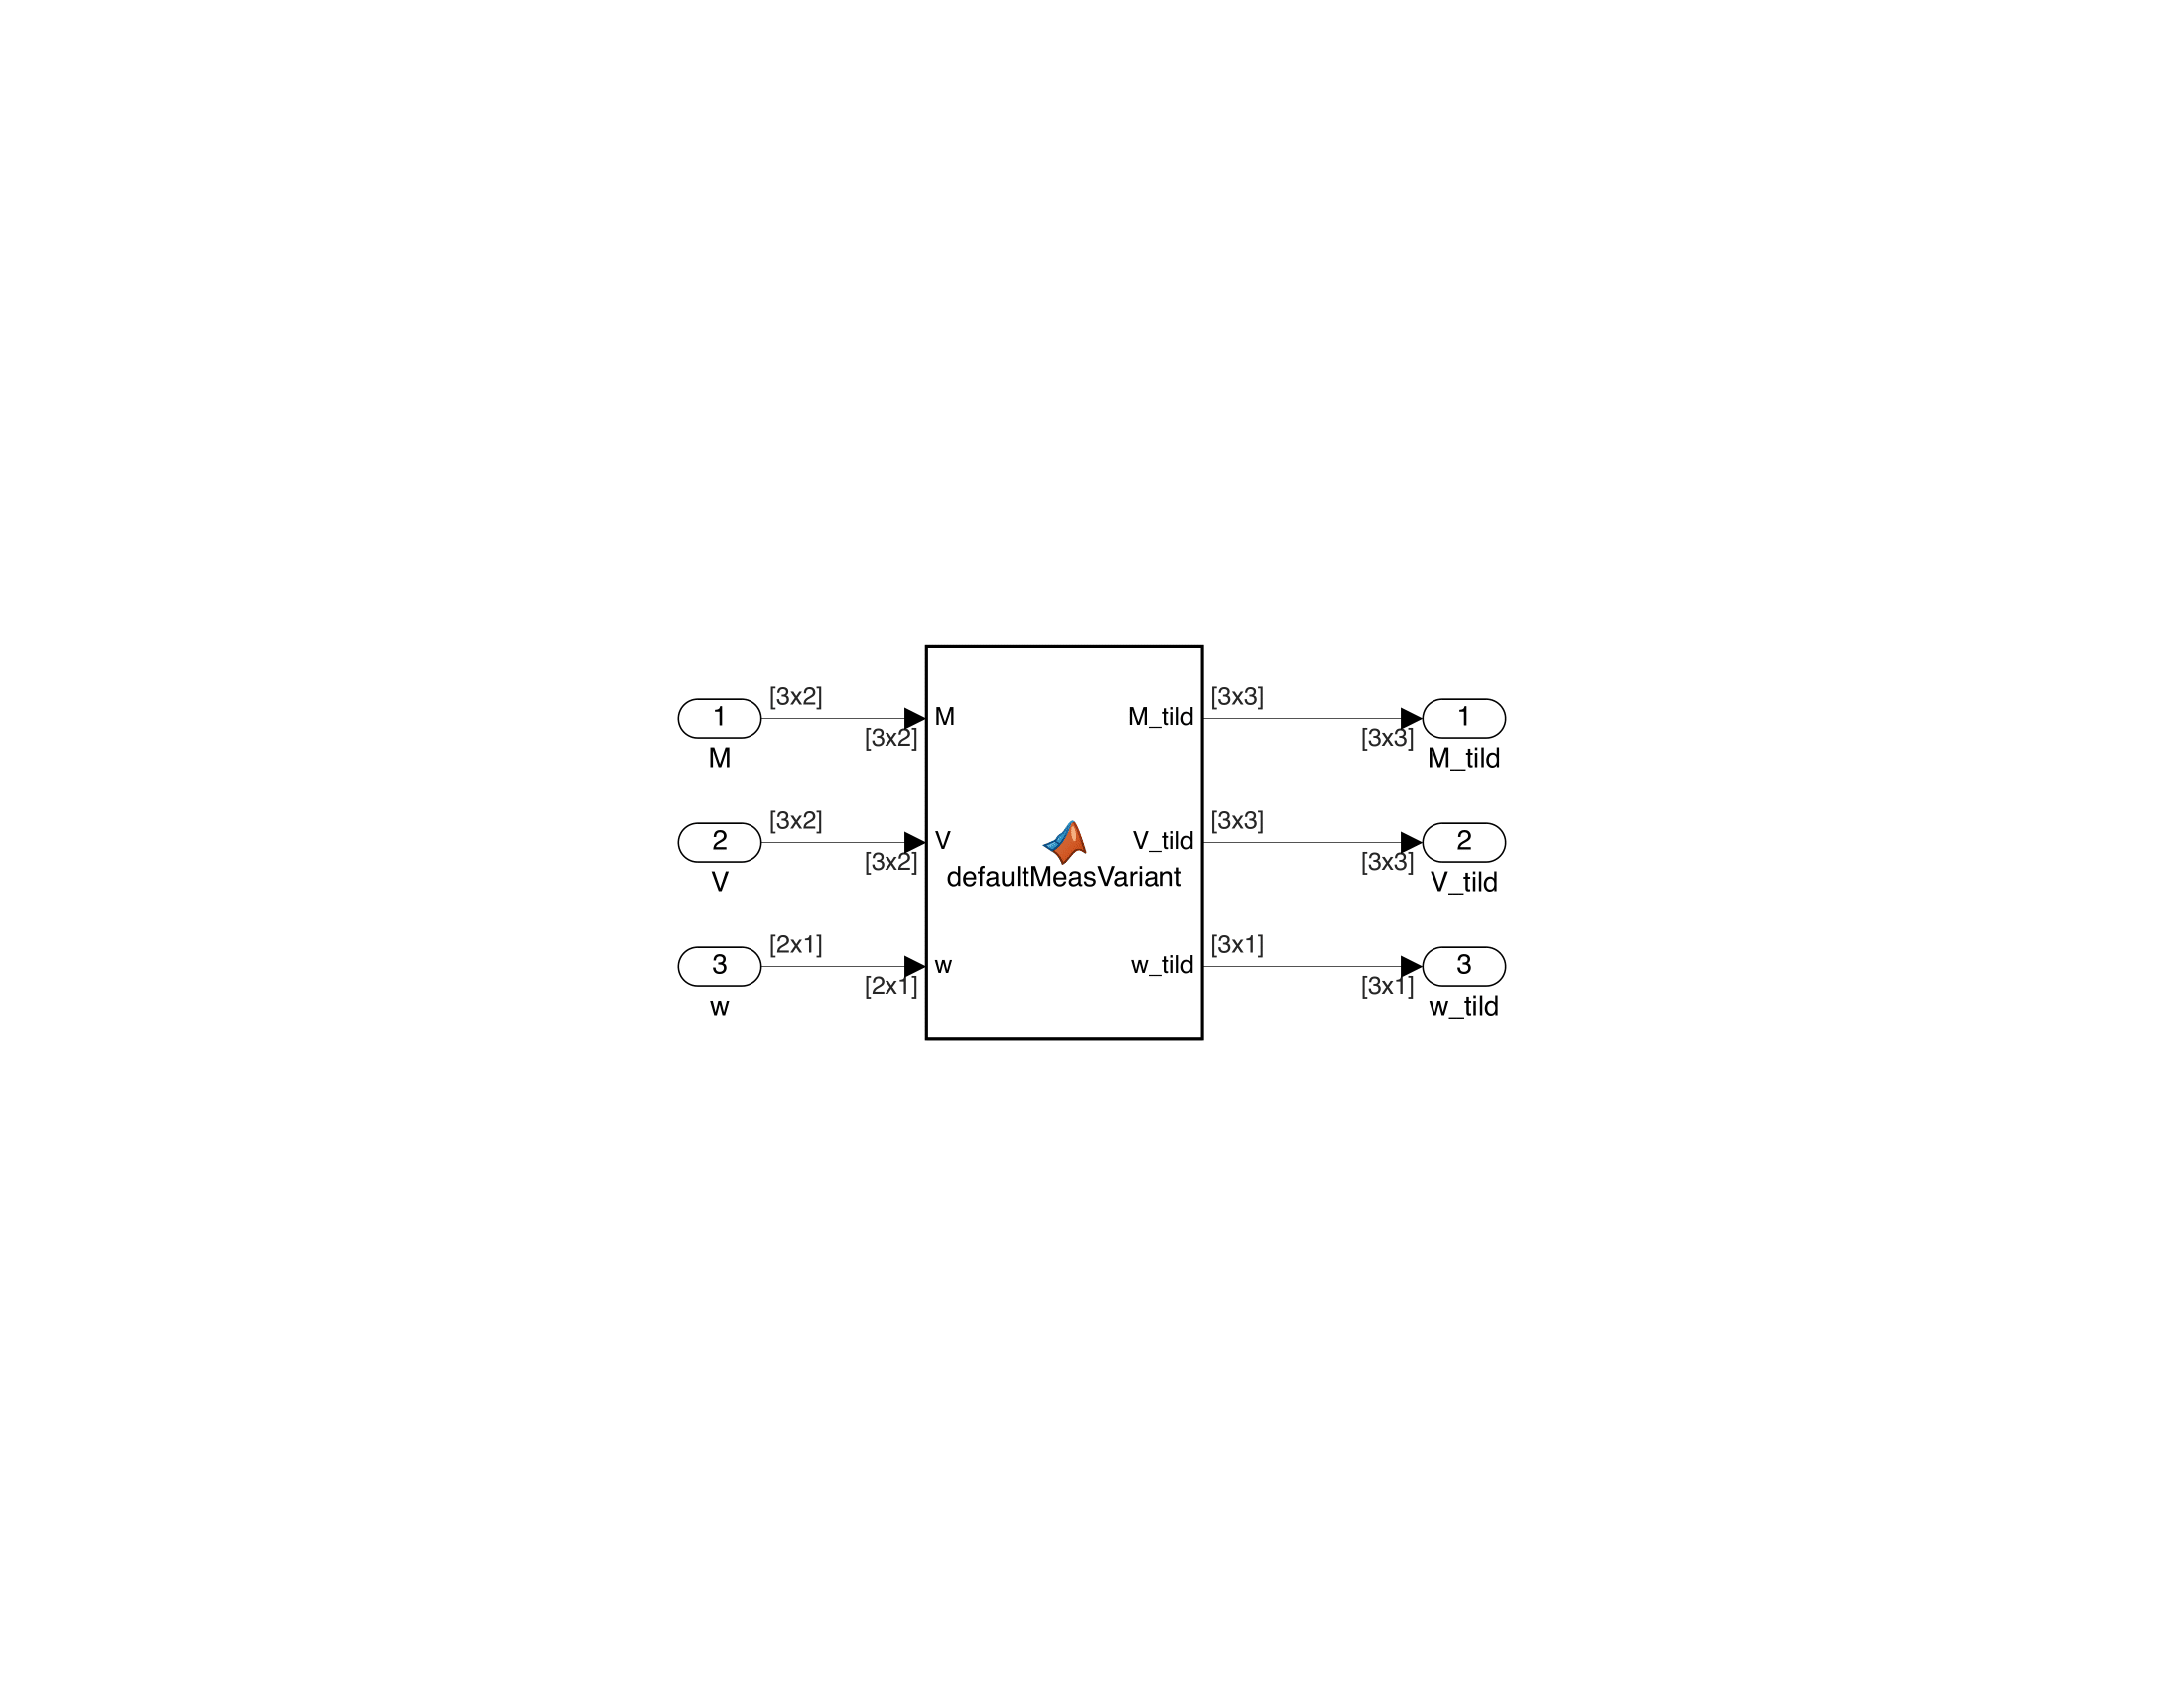
\includegraphics[trim={8cm 5cm 8cm 5cm},clip,width = 12cm]{Images/PS6/feedthrough_meas.png}
    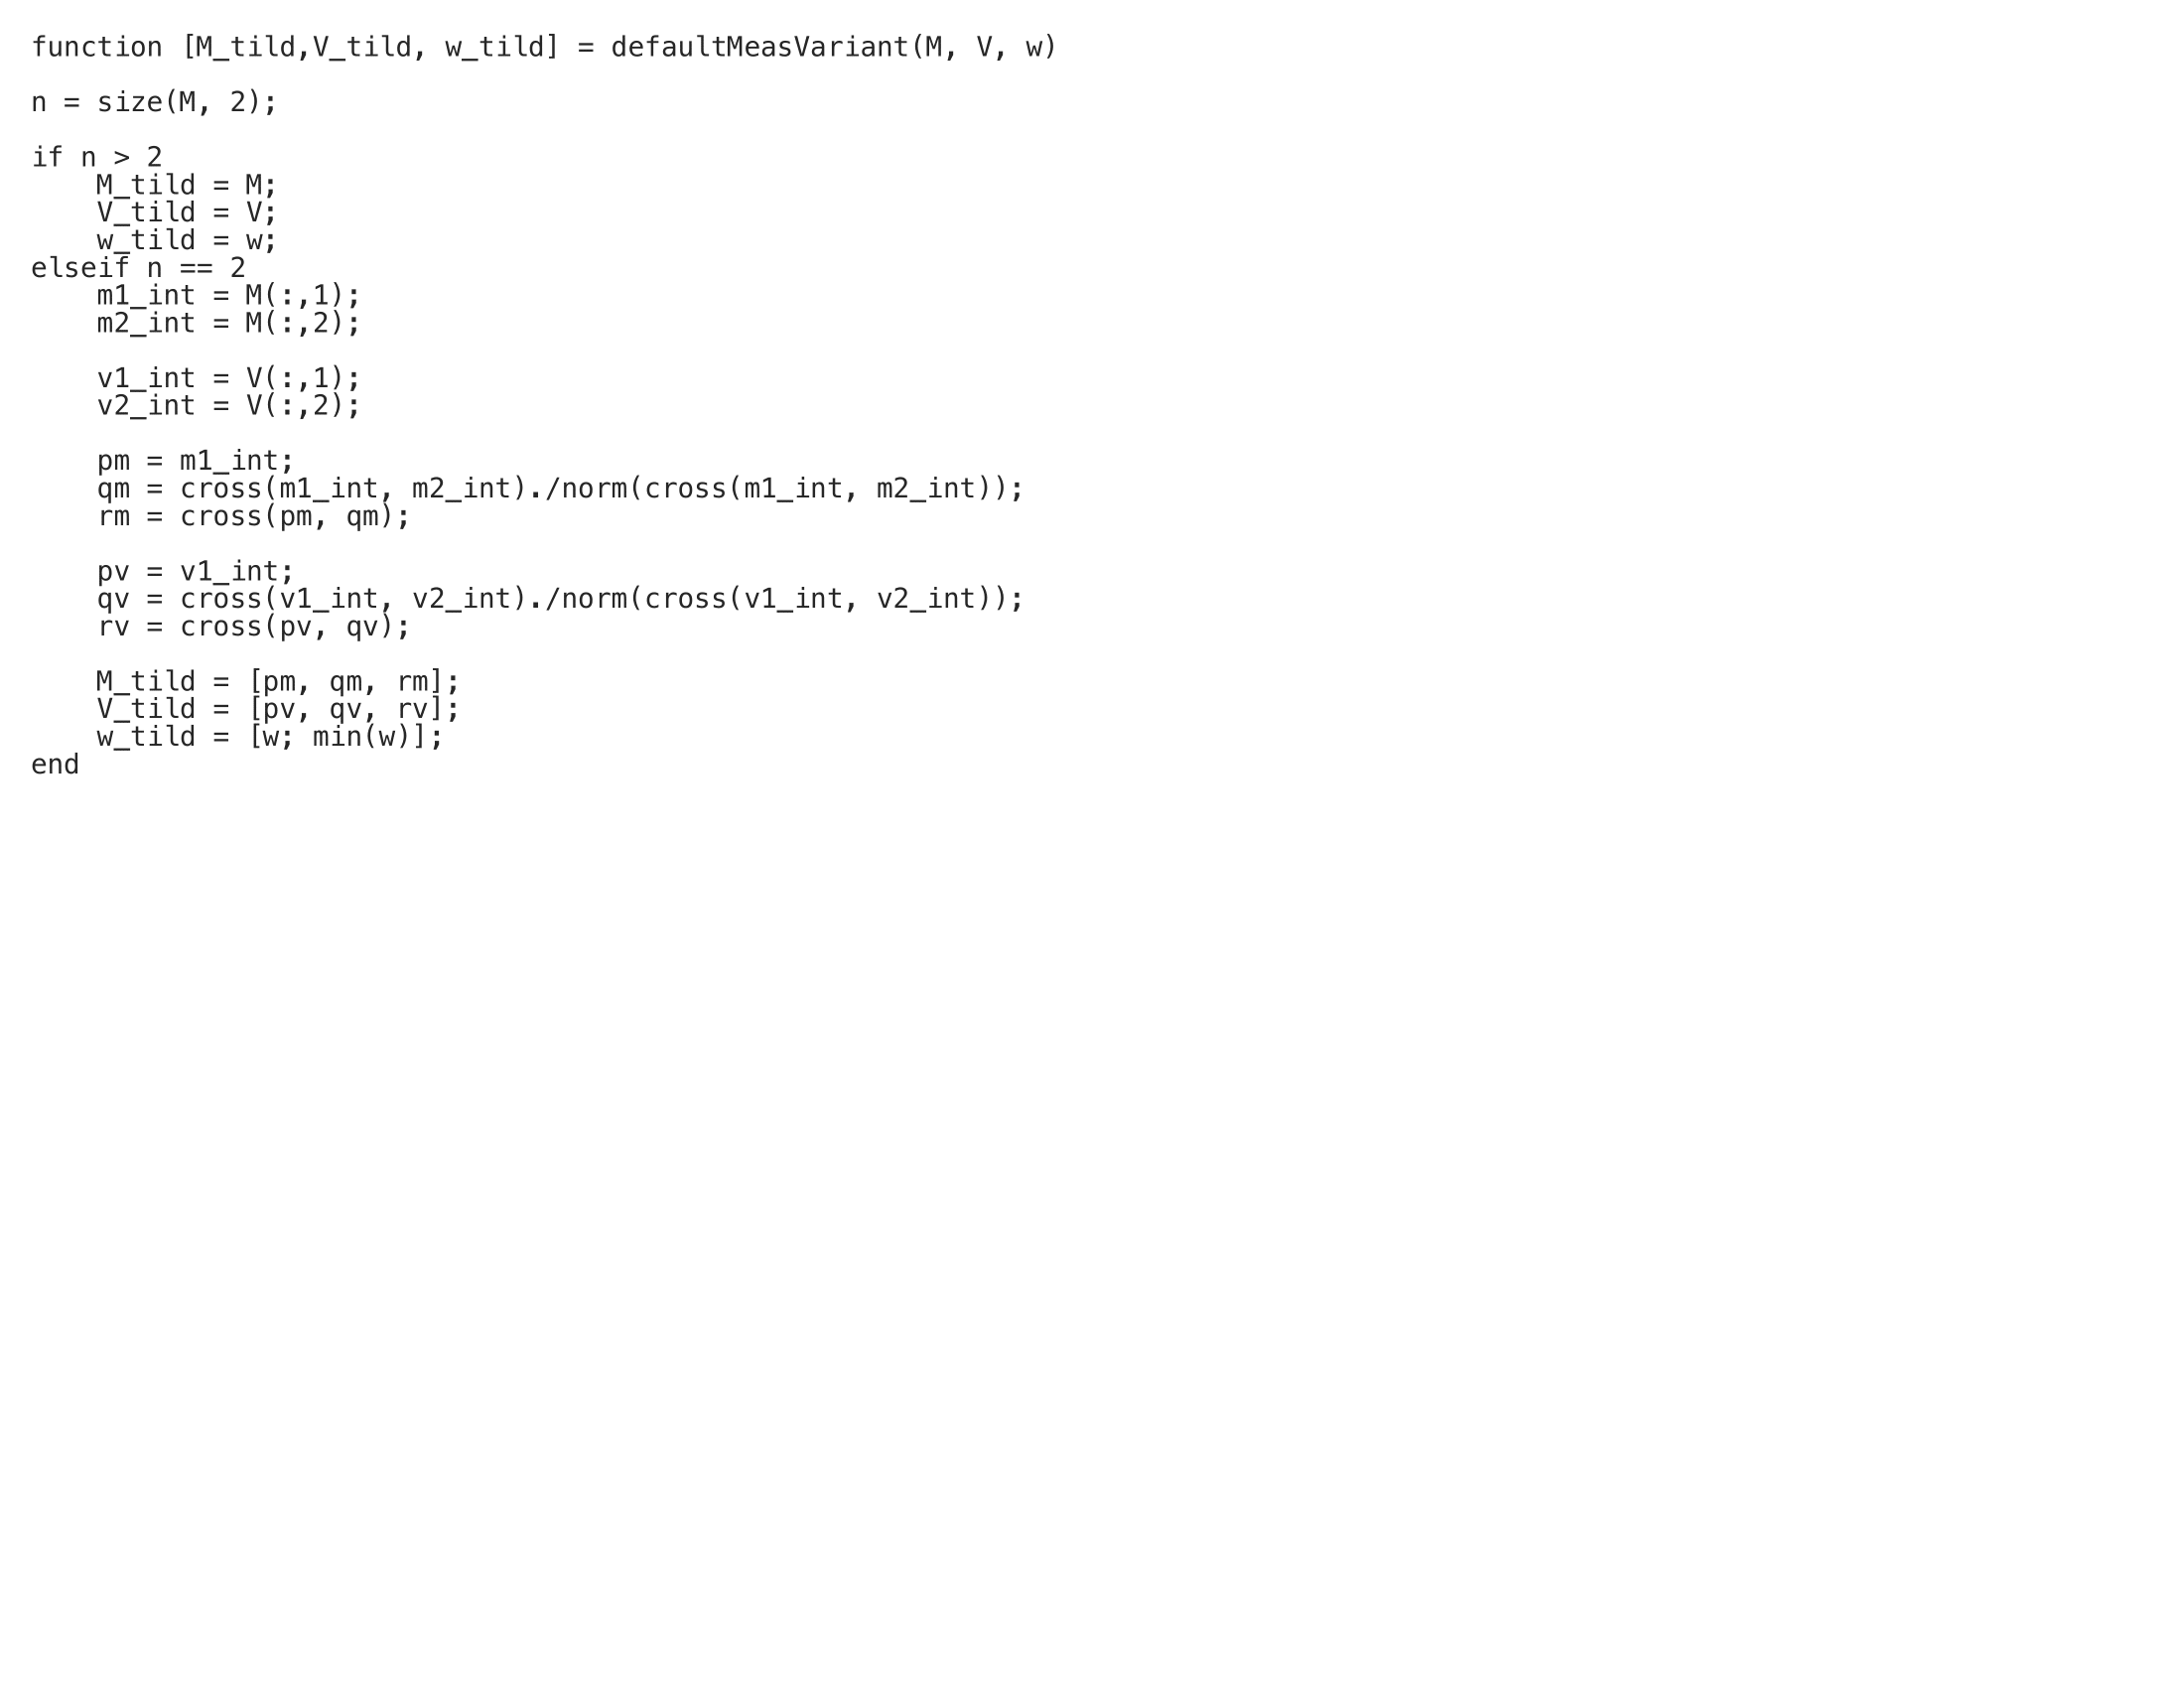
\includegraphics[trim={0cm 10cm 10cm 0cm},clip,width = 15cm]{Images/PS6/feedthrough_meas_code.png}
    \caption{Model for Star Tracker Measurement Generation}
    \label{fig:feedthrough_meas}
\end{figure}

\begin{figure}[H]
    \centering
    \captionsetup{ justification = centering }
    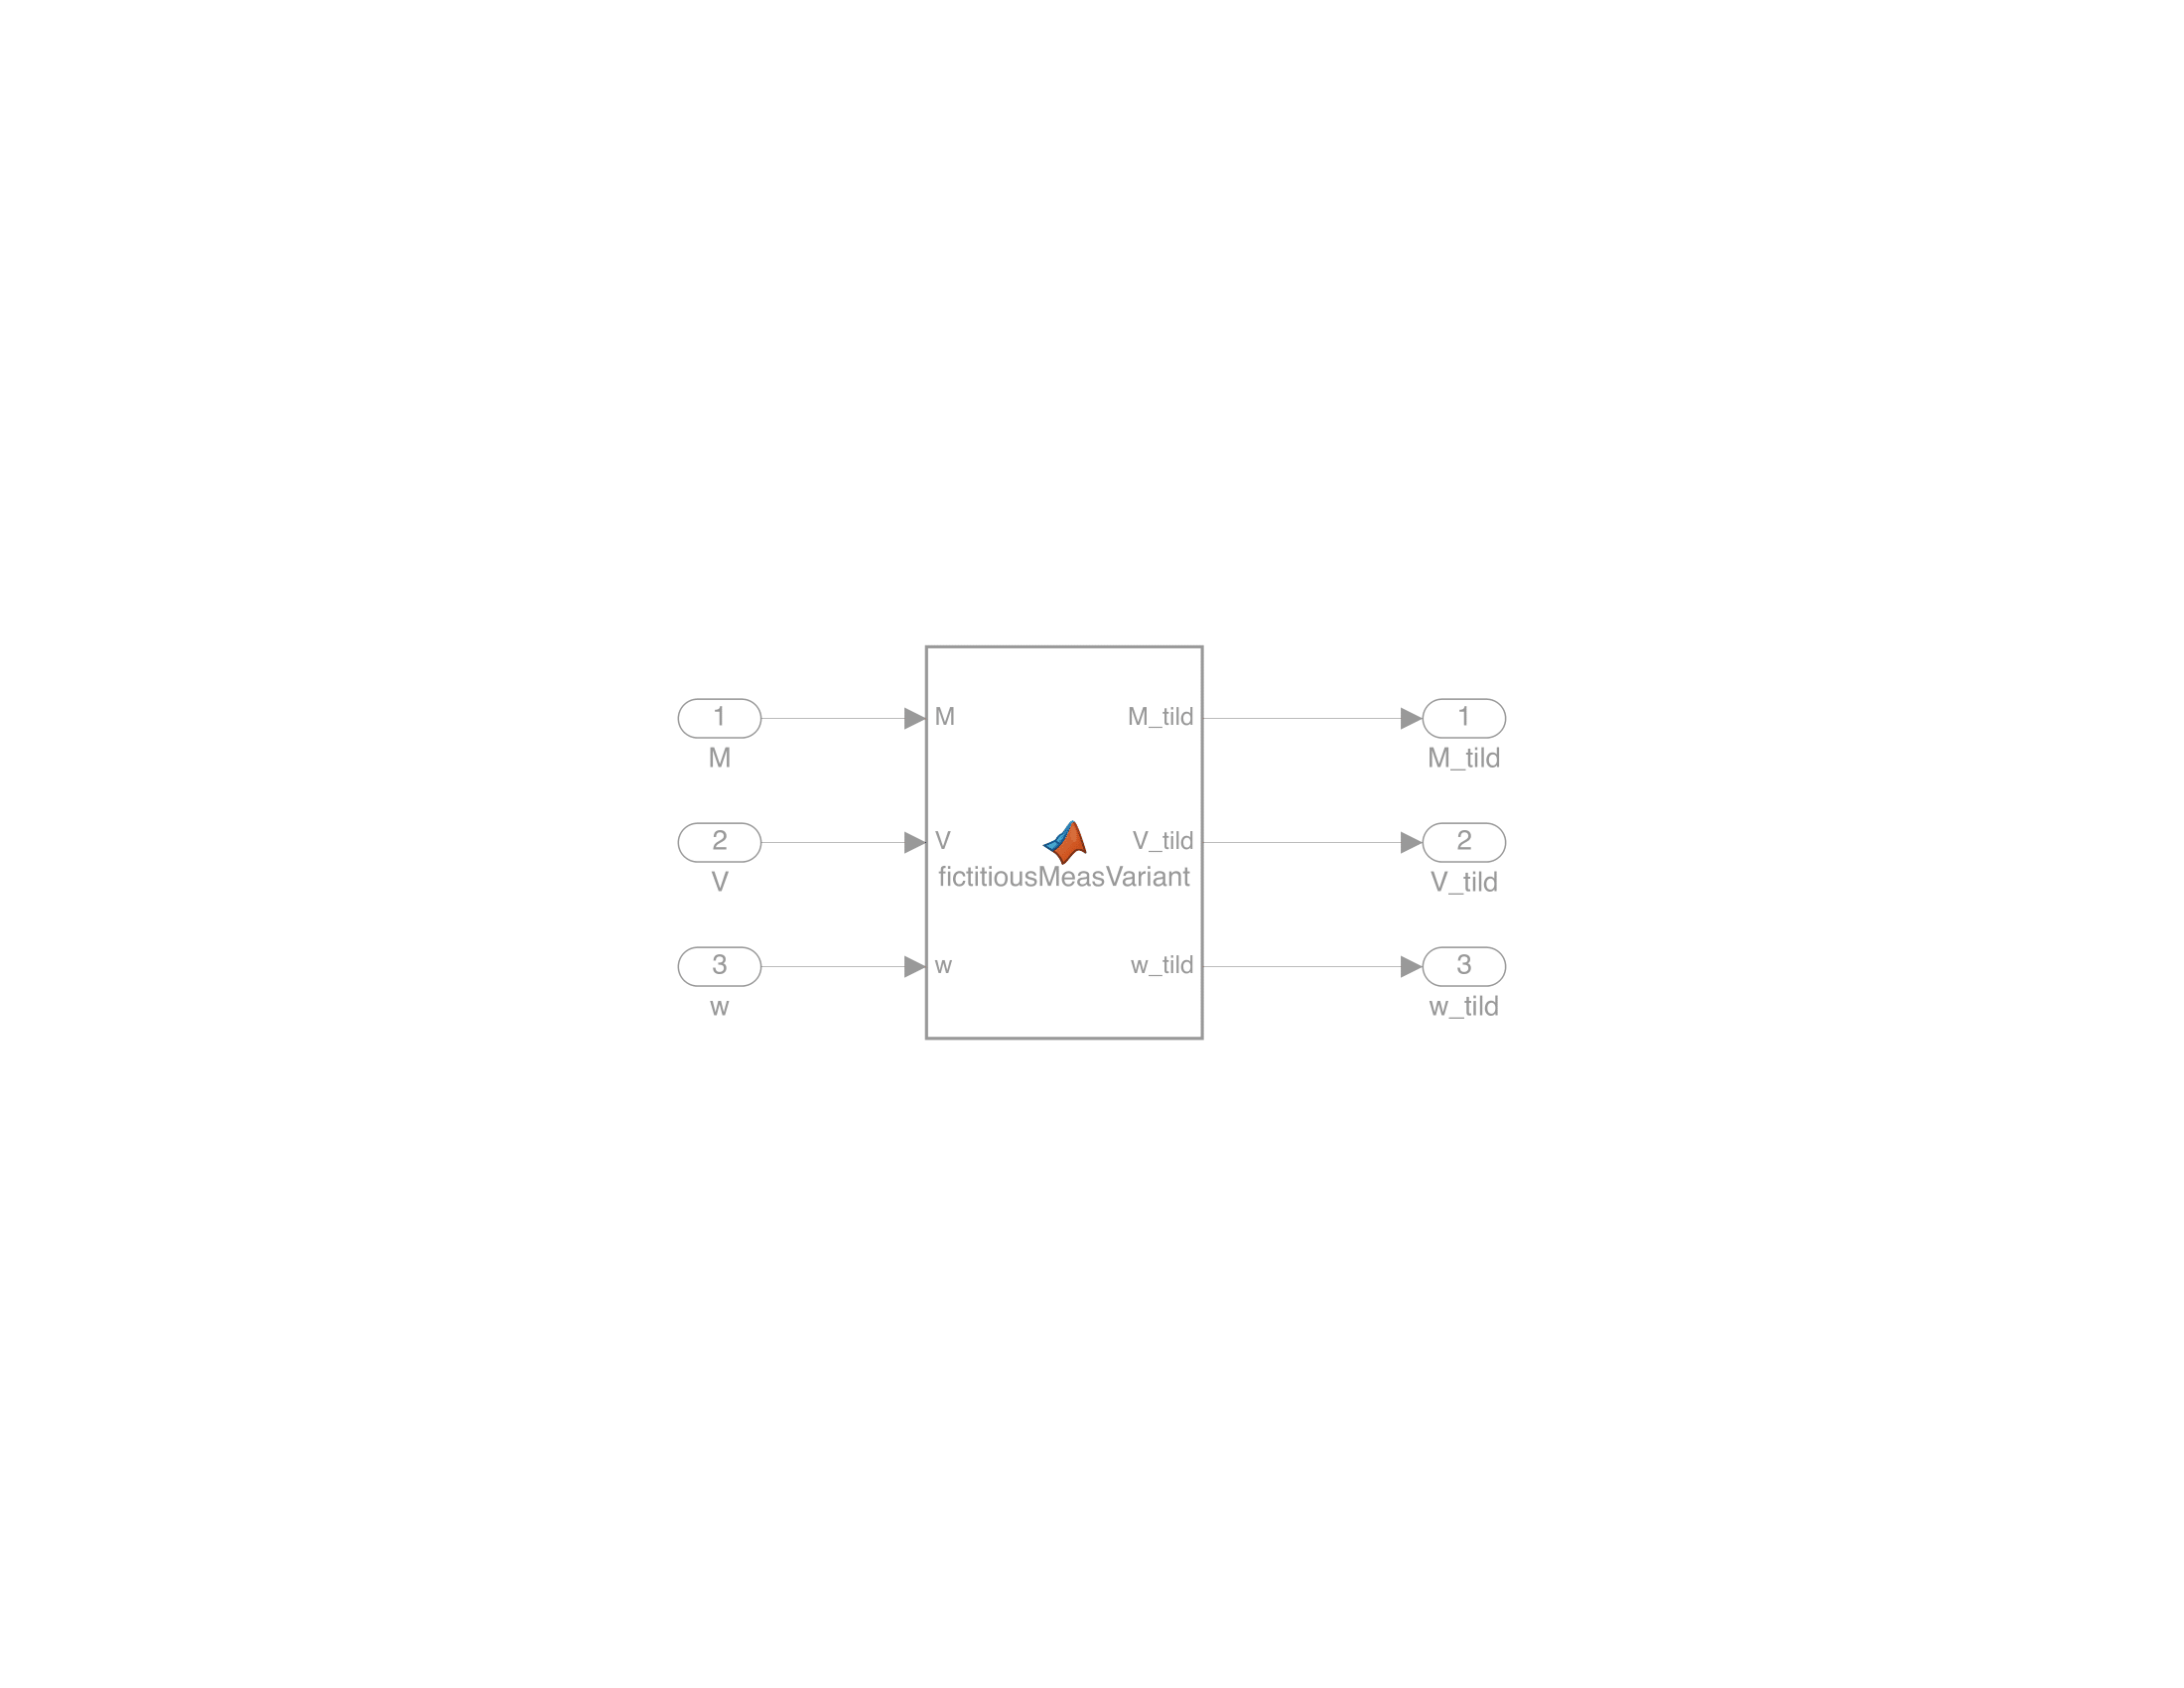
\includegraphics[trim={8cm 5cm 8cm 5cm},clip,width = 12cm]{Images/PS6/fict_meas.png}
    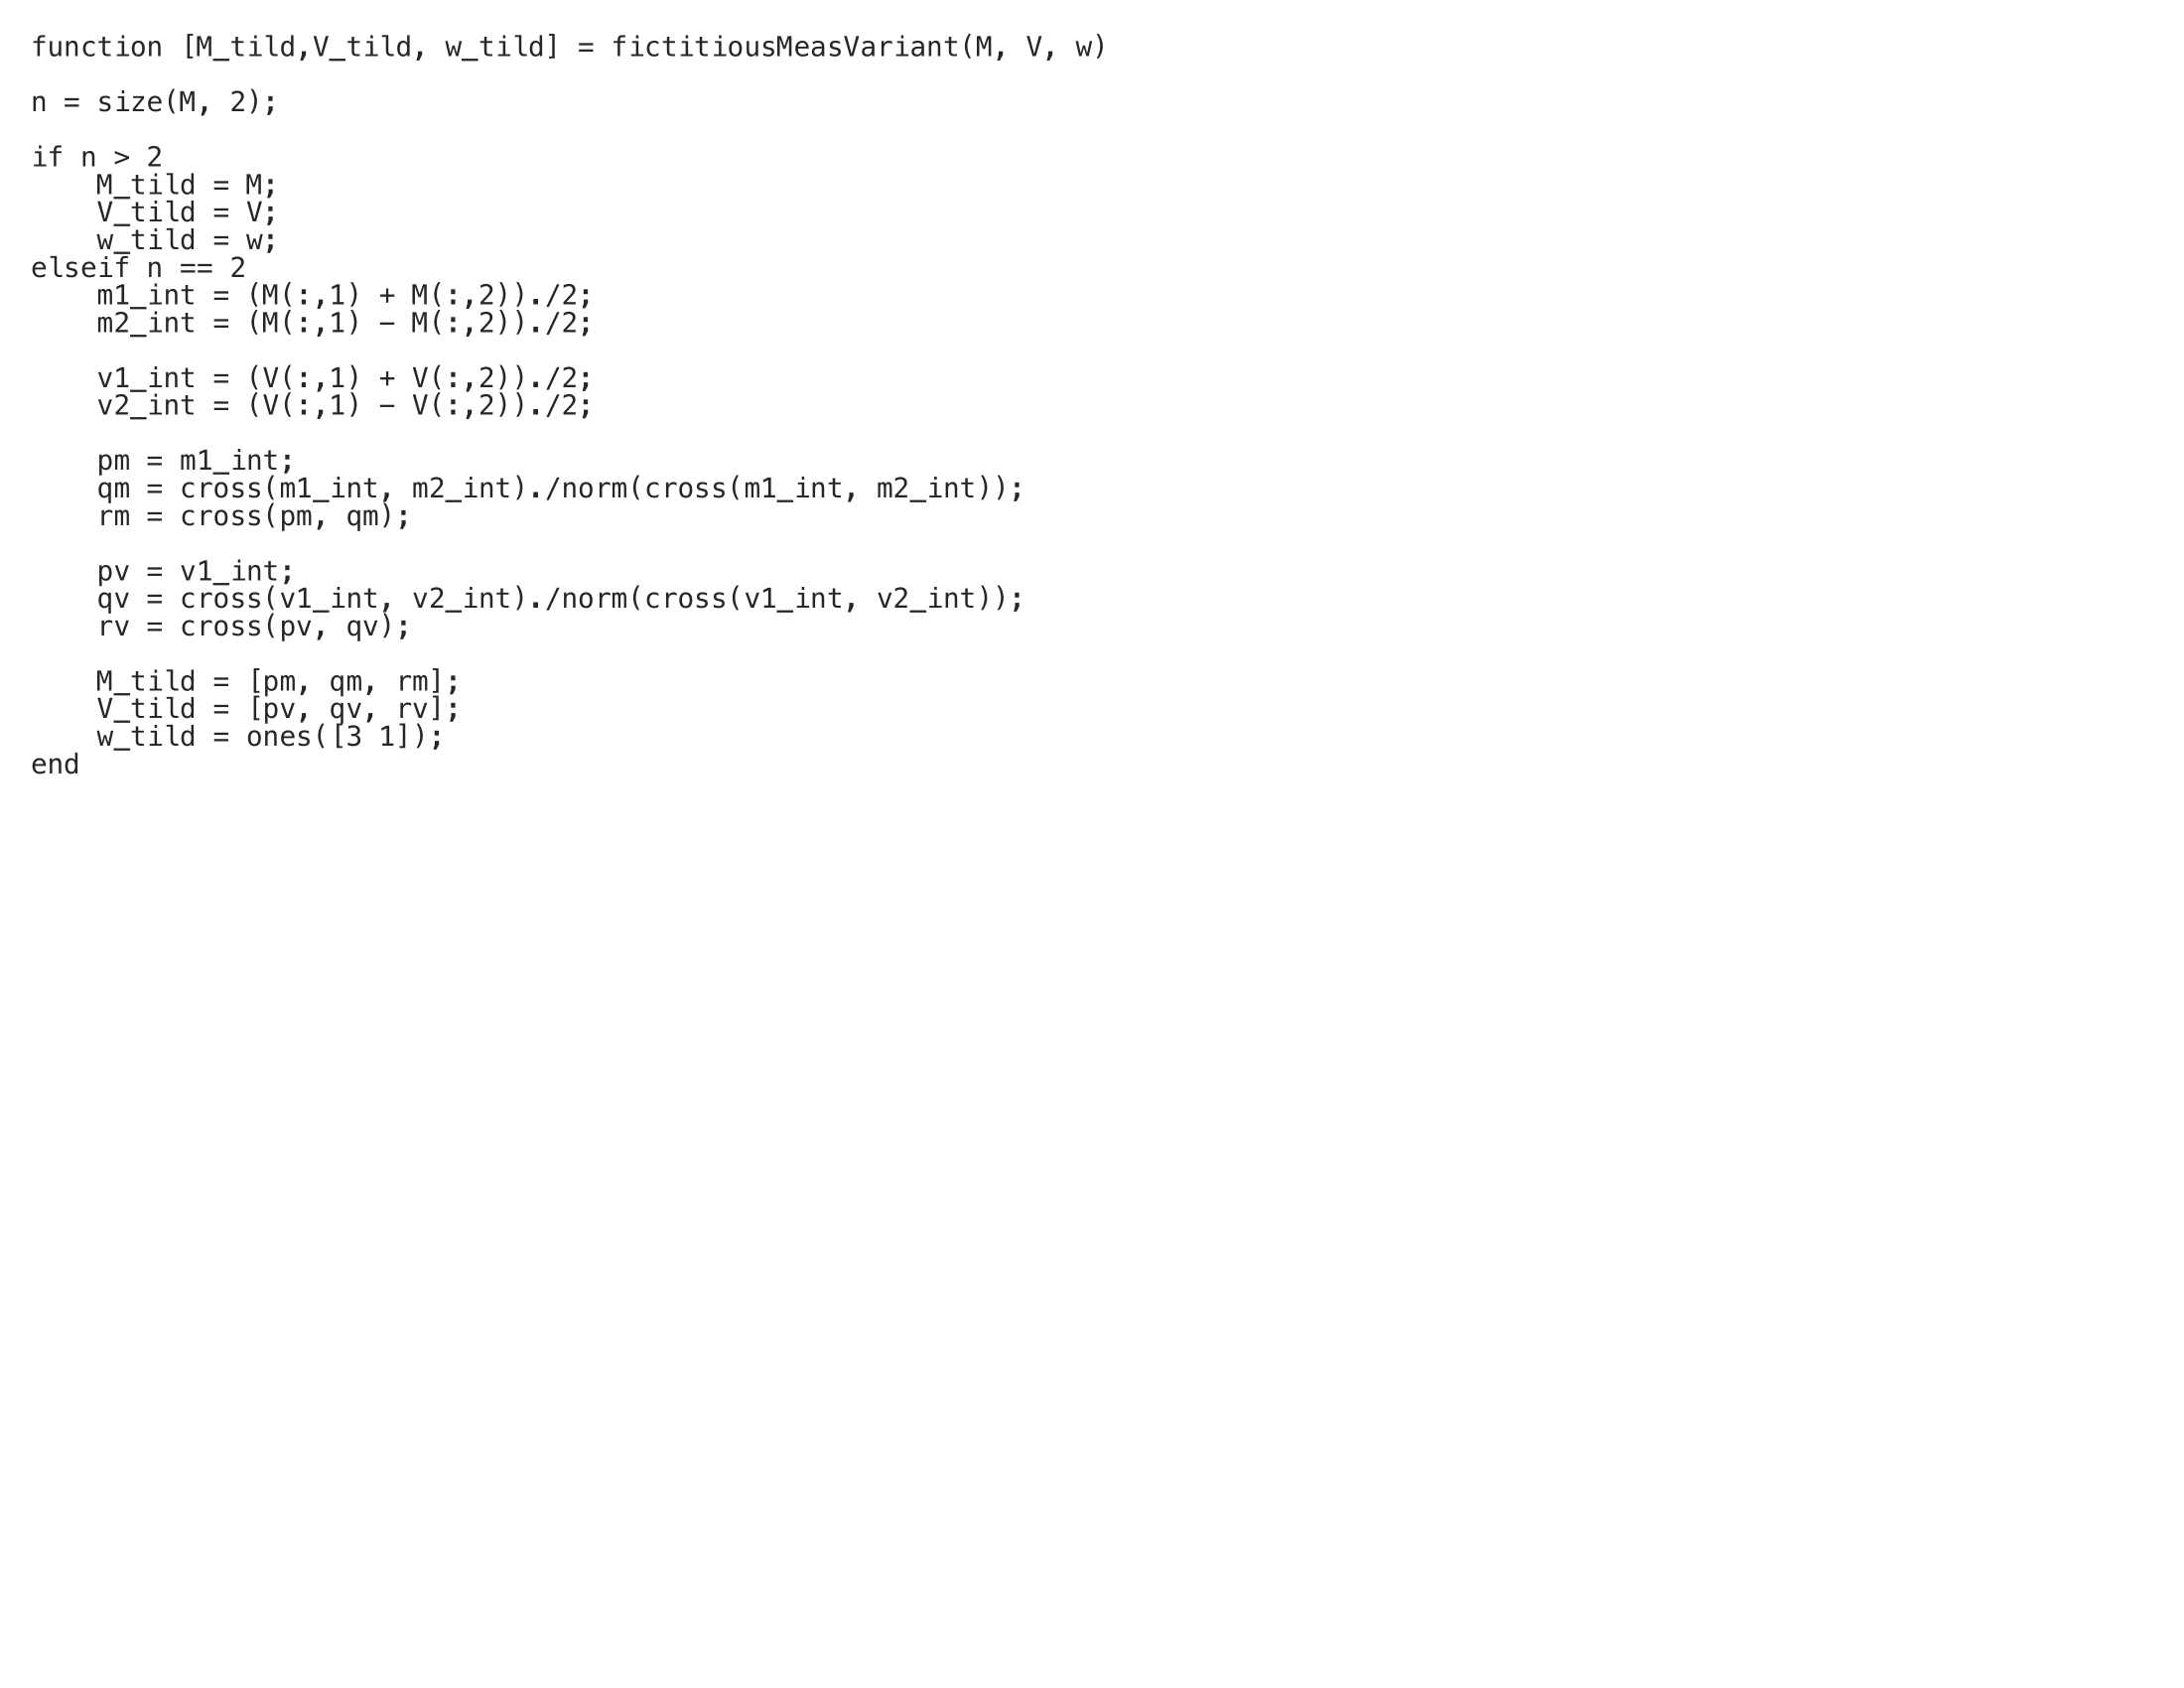
\includegraphics[trim={0cm 10cm 10cm 0cm},clip,width = 15cm]{Images/PS6/fict_meas_code.png}
    \caption{Model for Star Tracker Measurement Generation}
    \label{fig:fictitious_meas}
\end{figure}

\subsection{Problem 5 - Assume a certain set of sensors. In general, a number of unit = vectors and angular velocities can be considered as measurements.}

\subsubsection{Implement the deterministic attitude determination algorithm discussed in class and its variant which uses fictitious measurements to spread the errors across the measurements}

The deterministic attitude determination method was implemented using the model shown in Figure \ref{fig:det_attitude}.

\begin{figure}[H]
    \centering
    \captionsetup{ justification = centering }
    \includegraphics[trim={0.25cm 3cm 0.25cm 3cm},clip,width = 15cm]{Images/PS6/.png}
    \caption{Model for Star Tracker Measurement Generation}
    \label{fig:det_attitude}
\end{figure}

\subsubsection{Implement the statistical attitude determination algorithm discussed in class (q-method)}

\subsubsection{Implement angular velocity measurements and the reconstruction of the attitude from those (through kinematic equations coded identically to ground truth but replicated in the spacecraft on- board computer)}

\subsection{Problem 6 - Plot the resulting estimated attitude in the absence of sensor errors. Show that it is identical to the true attitude (except for numerical errors).}